\section{IAQ a IEQ}

Tato sekce vymezuje pojmy IAQ a IEQ, jejich jednotlivé složky a vzájemný vztah.

\FloatBarrier
\subsection{IAQ}
Začneme pojmem IAQ, který je podmnožinou pojmu IEQ (obr. \ref{obr:vztah_ieq_a_iaq}).

\begin{figure}[htbp!]
  \caption{Vztah mezi IEQ a IAQ}
	\label{obr:vztah_ieq_a_iaq}

	\centerfirst
	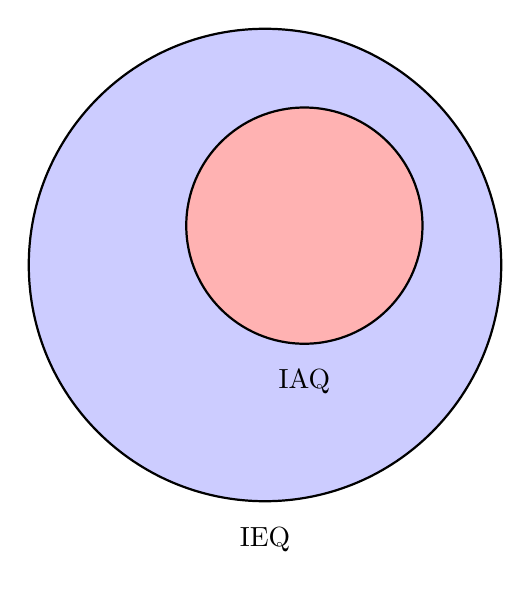
\begin{tikzpicture}
		% Množina IEQ
		\draw[thick, fill=blue!20] (0,0) circle (3cm) node[below] at (0,-3.2) {IEQ};
		
  % Množina IAQ
		\draw[thick, fill=red!30] (0.5,0.5) circle (1.5cm) node[below] at (0.5,-1.2) {IAQ};
	\end{tikzpicture}

\footnotesize Zdroj: vlastni zpracování
\end{figure}

Pojem IAQ je zkratkou pro vnitřní kvalitu ovzduší. IAQ představuje soubor veličin vztahujících se ke kvalitě vnitřního ovzduší. Řada obsažených veličin se uplatňuje i pro hodnocení kvality vnějšího ovzduší.
WHO (World Health Organization) vymezuje kvalitu ovzduší pomocí úrovní znečisťujících látek PM\textsubscript{2.5}\footnote{Particulate Matter $2.5\,\mu\text{m}$}, PM\textsubscript{10}\footnote{Particulate Matter $10\,\mu\text{m}$}, O\textsubscript{3} (Ozón), NO\textsubscript{2} (Oxid dusičitý), SO\textsubscript{2} (Oxid siřičitý) a CO (Oxid uhelnatý). Všechny zmíněné veličiny jsou znečisťující látky, které mají negativní vliv na člověka \parencite{worldhealthorganizationWHOGlobalAir2021}.

Na webu Úřadu pro ochranu životního prostředí USA\footnote{www.epa.gov} lze najít další znečisťující látky jako jsou radon, VOC (Volatile Organic Compounds), plíseň, bakterie, viry, pesticidy, cigaretový kouř a další látky, například aerosoly. Mezi významné znečišťující látky patří zejména VOC a radon. VOC jsou plyny, které se uvolňují z některých pevných či kapalných látek. Mohou způsobovat podráždění nosu a očí, bolesti hlavy a nevolnost, poškození jater, ledvin a CNS (centrální nervové soustavy), dokonce i rakovinu. \parencite{usepaIndoorPollutantsSources2015}
Součástí IAQ je také CO\textsubscript{2}, které při vysokých koncentracích přispívá k zhoršeným kognitivním schopnostem a stresu\parencite{dengImpactIndoorAir2024}.

\FloatBarrier
Jednotlivé znečišťující látky mají různě závažné negativní účinky na lidské zdraví. Jejich přehled shrnuje tabulka~\ref{tab:znecistujici-latky-ucinky}. Částice PM\textsubscript{2.5} a PM\textsubscript{10} jsou přitom definovány svým aerodynamickým průměrem (2,5 a 10\,$\mu\text{m}$) a~díky své velikosti mohou pronikat hluboko do dýchacího ústrojí, v~případě nejjemnějších frakcí až do krevního řečiště.

\begin{table}[!htbp]

\begin{center}
\footnotesize
\renewcommand{\arraystretch}{1.2}
\caption{Hlavní zdravotní účinky vybraných znečišťujících látek}\label{tab:znecistujici-latky-ucinky}
\begin{tabularx}{\textwidth}{p{2.0cm} X p{3.2cm}}
\toprule
\textbf{Látka} & \textbf{Hlavní zdravotní účinky} & \textbf{Zdroj} \\
\midrule
PM\textsubscript{2.5}, PM\textsubscript{10} & Pronikání do plic a~krevního řečiště, mj. astma, ischemická choroba srdeční, srdeční selhání a~chronická obstrukční plicní nemoc (CHOPN). & \parencite{usepaIndoorPollutantsSources2015} \\
O\textsubscript{3} & Pokles plicní kapacity, zánětlivá onemocnění plic, narušení vývoje plic, více hospitalizací a~zvýšená úmrtnost. & \parencite{worldhealthorganizationWHOGlobalAir2021} \\
NO\textsubscript{2} & Podráždění dýchacích cest, oxidační stres, endoteliální dysfunkce a~srdečně-cévní rizika, rozvoj astmatu a~CHOPN. & \parencite{usepaNitrogenDioxidesImpact2014} \\
SO\textsubscript{2} & Dráždění dýchacích cest a~sliznic, kašel, zhoršení astmatu, chronická bronchitida, kardiovaskulární rizika. & \parencite{usepaSulfurDioxideBasics2016} \\
CO & Vazba na hemoglobin a~snížení přenosu kyslíku, bolesti hlavy, závratě, při vyšší expozici bezvědomí až smrt. & \parencite{usepaBasicInformationCarbon2016} \\
\bottomrule
\end{tabularx}

\footnotesize \textit{Zdroj:} Vlastní zpracování na základě uvedených zdrojů.
\end{center}
\end{table}

\FloatBarrier
\subsubsection{VOC}
VOC je zkratka anglického označení \textit{volatile organic compounds}.
VOC zahrnují široké spektrum látek. Podle \textcite{lancea.wallaceVOLATILEORGANICCOMPOUNDS1991} mezi běžně se vyskytující látky patří například aromatické uhlovodíky (benzen, toluen, ethylbenzen, xylen, styren), chlorované uhlovodíky (chloroform, dichlormethan, trichloroethylen, tetrachlorethylen) a terpeny (limonen, $\alpha$-pinen).

\FloatBarrier
\subsection{IEQ}
IEQ je nadřazeným pojmem pro IAQ. K veličinám měřeným v IAQ přidává veličiny jako jsou \textit{tepelný komfort}, \textit{vizuální komfort} a \textit{akustický komfort}. Tyto kategorie společně s IAQ tvoří prostředí, ve kterém se člověk pohybuje \parencite{dengImpactIndoorAir2024}.

Je důležité si všimnout, že ne všechny veličiny, které IEQ nově přináší, jsou dobře senzoricky měřitelné. Zejména veličiny jako \textit{oblečení}, \textit{soukromí}, \textit{oslnění}, \textit{výhled} a \textit{design budovy} jsou obtížně měřitelné a často subjektivní. Proto tyto veličiny dále nejsou předmětem práce.

\FloatBarrier
\subsubsection{Tepelný komfort}
Teplotu můžeme rozdělit na teplotu ovzduší a teplotu povrchu. Především teplota ovzduší je pro člověka velmi důležitá. Významně ovlivňuje produktivitu člověka a špatné tepelné podmínky mohou zvyšovat únavu a diskomfort, zejména při vysoké teplotě a vysoké vlhkosti. \parencite{dengImpactIndoorAir2024} 

Vlhkostí je myšlena zejména vlhkost relativní. Ta vyjadřuje, do jaké míry je vzduch nasycen vodou. Množství vody, které je vzduch schopný pojmout, závisí na jeho teplotě. \parencite{dengImpactIndoorAir2024} Čím vyšší teplota, tím větší množství vody může vzduch obsahovat. \parencite{VlhkostVzduchu2024}

Rychlost vzduchu ovlivňuje vnímaný tepelný komfort a pocitovou teplotu. Při vyšší rychlosti vzduchu dochází k většímu ochlazování těla a tím i k nižšímu vnímání teploty. \parencite{dengImpactIndoorAir2024}
\FloatBarrier
\subsubsection{Vizuální komfort}
Vizuální komfort je spolu s tepelným komfortem nejdůležitějším faktorem IEQ.

Světlo můžeme rozdělit na přirozené a umělé. Přirozené světlo je důležité pro regulaci cirkadiánních rytmů, které řídí spánek, náladu a kognitivní funkce. Přirozené světlo má prokazatelně pozitivní vliv na zdraví, pozornost a produktivitu. Ve studii mezi žáky bylo zjištěno, že žáci, kteří měli větší přístup k přirozenému světlu, měli lepší výsledky v matematice a čtení o zhruba 20 \% než žáci, kteří měli vyšší podíl umělého osvětlení. \parencite{dengImpactIndoorAir2024} 

Intenzita osvětlení může ovlivňovat učení, paměť a kreativitu. Vysoká intenzita přispívá k lepší paměti a učení, zatímco nízká intenzita podporuje kreativitu. Vizuální komfort je v praxi nejčastěji monitorován právě pomocí intenzity osvětlení. \parencite{dengImpactIndoorAir2024}

Rovnoměrnost osvětlení je důležitá pro vizuální komfort. Nerovnoměrné osvětlení může způsobovat únavu očí a diskomfort. \parencite{dengImpactIndoorAir2024}

Barevná teplota (CCT - Correlated Color Temperature) je měřítkem barevného odstínu světla. Vyšší CCT (chladnější světlo) může zlepšit pozornost a produktivitu, zatímco nižší CCT (teplejší světlo) může podporovat relaxaci a kreativitu. \parencite{dengImpactIndoorAir2024}

Oslňování způsobené světelnými zdroji či odrazy od povrchů může způsobovat diskomfort a snižovat vizuální komfort. \parencite{dengImpactIndoorAir2024}

\FloatBarrier
\subsubsection{Akustický komfort}
Hluk způsobuje rozptýlení, nepohodu a únavu. Zejména v otevřených kancelářích má největší vliv na produktivitu ze všech faktorů IEQ. \parencite{dengImpactIndoorAir2024}

V kombinaci s teplotou má hluk výrazný vliv na pracovní paměť, přičemž hluk působí na pracovní paměť výrazněji než teplota. \parencite{dengImpactIndoorAir2024} 

Ve výzkumu provedeném ve třídách bylo zjištěno, že vysoká míra hluku způsobuje únavu, bolesti hlavy a další nepříznivé stavy. \parencite{dengImpactIndoorAir2024}

Změna hluku o 3,9 dB odpovídá změně teploty o 1 \textdegree C. \parencite{dengImpactIndoorAir2024}


\FloatBarrier
\subsection{Standardy}

Tato část vymezuje jednotky používané pro měřené veličiny IEQ a legislativu a standardy, které pro vnitřní prostředí stanovují limitní hodnoty.

\FloatBarrier
\subsubsection{Jednotky}
IEQ a IAQ zahrnují mnoho různých veličin, které se měří v různých jednotkách. Proto je důležité se s těmito jednotkami seznámit a pochopit, jaké jsou mezi nimi rozdíly a jak je správně používat. V textu se objevují jednotky \textit{ppm}, \textit{ppb}, \textit{$\mu\text{g}*m^{-3}$}, \textit{°C}, \textit{K}, \textit{\%}, \textit{dB} a další. Přiřazení jednotek k jednotlivým veličinám IEQ a~jeho upřesnění shrnuje tabulka~\ref{tab:ieq-jednotky}.\parencite{dengImpactIndoorAir2024}

Jednotky lze rozdělit do tří kategorií. První kategorií jsou jednotky pro poměrové koncentrace, většinou \textit{ppm} (parts per million) a \textit{ppb} (parts per billion), které vyjadřují poměr množství měřené látky k celkovému množství směsi (vzduchu). Druhou kategorií jsou jednotky pro hmotnostní koncentrace, jako je \textit{$\mu\text{g}*m^{-3}$} (mikrogramy na metr krychlový), vyjadřující hmotnost měřené látky v určitém objemu vzduchu. Třetí kategorií jsou jednotky pro fyzikální veličiny prostředí, jako jsou \textit{°C} (stupně Celsia) a \textit{K} (Kelvin) pro teplotu, \textit{\%} pro relativní vlhkost a \textit{dB} (decibel) pro hluk.\parencite{worldhealthorganizationWHOGlobalAir2021}

Jednotky ppm a ppb se dají převádět na $\mu\text{g}*m^{-3}$, k čemuž je nutné znát podmínky měření (T, p) a molární hmotnost látky. Zda tento převod dává smysl, závisí na konkrétní látce.\parencite{worldhealthorganizationWHOGlobalAir2021}

\begin{table}[!tbp]

\begin{center}
\footnotesize
\renewcommand{\arraystretch}{1.15}
\caption{Shrnutí jednotek pro vybrané veličiny IEQ}\label{tab:ieq-jednotky}
\begin{tabularx}{\textwidth}{p{2.2cm} p{3.0cm} p{1.8cm} p{1.8cm} >{\raggedright\arraybackslash}X}
\toprule
\textbf{Kategorie IEQ} & \textbf{Veličina} & \textbf{Značka} & \textbf{Jednotka} & \textbf{Poznámka /
  alternativa} \\
\midrule
Tepelná & Teplota vzduchu & $T$ & $^\circ$C & Alternativně K (např. v některých zdrojích/technických
listech). \\
Tepelná & Relativní vlhkost & RH & \% & --- \\
Tepelná & Rychlost proudění vzduchu & $v$ & m/s & Volitelné (pokud uvádíte v části tepelný komfort).
\\
\midrule
IAQ (plyny) & Oxid uhličitý / ekv. CO$_2$ & CO$_2$, eCO$_2$ & ppm & eCO$_2$ je často odhad senzoru;
pro převod ppm$\leftrightarrow$mg/m$^3$ je nutné znát podmínky (T, p). \\
IAQ (plyny) & Oxid uhelnatý & CO & mg/m$^3$ & Často i ppm; některé guideline uvádějí konverzní
faktory pro dané T/p. \\
IAQ (plyny) & Oxid dusičitý & NO$_2$ & $\mu$g/m$^3$ & Často i ppb; převody závisí na T/p. \\
IAQ (plyny) & Ozon & O$_3$ & $\mu$g/m$^3$ & Často i ppb; převody závisí na T/p. \\
IAQ (plyny) & Oxid siřičitý & SO$_2$ & $\mu$g/m$^3$ & Často i ppb; převody závisí na T/p. \\
IAQ (VOC) & Celkové VOC & TVOC & ppb & U senzorů typicky ppb; význam TVOC závisí na
metodě/kalibraci. \\
IAQ (VOC) & Celkové VOC & TVOC & $\mu$g/m$^3$ & V laboratorních studiích/limitech se často uvádí i
$\mu$g/m$^3$; nepřevádět „naslepo" bez definice směsi. \\
IAQ (částice) & PM$_{2.5}$ & PM$_{2.5}$ & $\mu$g/m$^3$ & Hmotnostní koncentrace; ppm se pro PM běžně
nepoužívá. \\
IAQ (částice) & PM$_{10}$ & PM$_{10}$ & $\mu$g/m$^3$ & Hmotnostní koncentrace; ppm se pro PM běžně
nepoužívá. \\
\midrule
Vizuální & Osvětlenost & $E$ & lx & --- \\
Vizuální & Korelovaná teplota chromatičnosti & CCT & K & Volitelné (pokud řešíte i spektrum/barvu
světla). \\
\midrule
Akustická & Hladina akustického tlaku (A-vážená) & $L_A$ & dB(A) & A-vážení (frekvenční vážení) pro
lepší vazbu na vnímání člověka; uvést, pokud možno, i metodu (např. LAeq). \\
Akustická & Hladina akustického tlaku (nevážená) & $L$ & dB & Méně běžné pro posuzování komfortu;
bez frekvenčního vážení. \\
\bottomrule
\end{tabularx}
\end{center}

\footnotesize Zdroj: \parencite{worldhealthorganizationWHOGlobalAir2021,osephg.allenAssociationsCognitiveFunction2016,calvoScalableIoTArchitecture2022,dengImpactIndoorAir2024,mcminnAWeightingMetric2013,marshIEC61672NewInternational2001}.
\end{table}

\FloatBarrier
\subsubsection{Legislativa}
Tato sekce uvádí přehled dokumentů (ČR, EU a WHO), které se vztahují k jednotlivým složkám IEQ, a shrnuje nejčastěji sledované veličiny a jejich referenční hodnoty. Práce se neomezuje pouze na legislativně či doporučeními vymezené ukazatele. Pokud některá doména IEQ není pokryta, jsou zahrnuty i další prakticky měřitelné parametry. Vše, co je vymezeno závazně či doporučeno, je při návrhu a interpretaci dat zohledněno.

Úplný přehled relevantních dokumentů (ČR, EU a WHO) a jejich pokrytí jednotlivých domén IEQ uvádí tabulka~\ref{tab:legislativa_ieq_dokumenty} v~příloze~\ref{app:legislativa}. Některé z~těchto dokumentů se vztahují pouze k~vnějšímu prostředí (např. vnější ovzduší nebo hluk), mohou však být relevantní i~pro vnitřní prostředí budov. Limitní a~doporučené hodnoty pro vybrané látky vnějšího ovzduší relevantní pro IAQ shrnuje tabulka~\ref{tab:iaqlimity_cr_eu_who} v~téže příloze. Tyto hodnoty se liší podle dokumentu a~doby průměrování.

V tabulce \ref{tab:indoor_limity_cr} jsou uvedeny limitní hodnoty chemických, fyzikálních a biologických ukazatelů pro vnitřní prostředí pobytových místností dle vyhlášky č.~43/2025~Sb.

\begin{table}[p]

\begin{center}
\setlength{\tabcolsep}{3pt}
\renewcommand{\arraystretch}{1.05}
\scriptsize
\caption{Limitní hodnoty pro vnitřní prostředí pobytových místností}\label{tab:indoor_limity_cr}
\begin{tabularx}{\textwidth}{@{}
>{\raggedright\arraybackslash}p{0.25\textwidth}
  >{\raggedright\arraybackslash}p{0.15\textwidth}
  >{\raggedright\arraybackslash}p{0.12\textwidth}
  X@{}}
\toprule
\textbf{Ukazatel} & \textbf{Jednotka} & \textbf{Limit} & \textbf{Poznámka} \\
\midrule
\multicolumn{4}{l}{\textit{Chemické ukazatele (hodinové limity)}} \\
NO$_2$ (oxid dusičitý) & $\mu$g/m$^3$ & 100 & — \\
CO (oxid uhelnatý) & $\mu$g/m$^3$ & 5\,000 & — \\
O$_3$ (ozón) & $\mu$g/m$^3$ & 100 & — \\
NH$_3$ (amoniak) & $\mu$g/m$^3$ & 70 & — \\
Benzen & $\mu$g/m$^3$ & 5 & — \\
Toluen & $\mu$g/m$^3$ & 300 & — \\
Suma xylenů & $\mu$g/m$^3$ & 200 & — \\
Styren & $\mu$g/m$^3$ & 40 & — \\
Ethylbenzen & $\mu$g/m$^3$ & 200 & — \\
Formaldehyd & $\mu$g/m$^3$ & 50 & — \\
Acetaldehyd & $\mu$g/m$^3$ & 200 & — \\
Trichlorethen & $\mu$g/m$^3$ & 25 & — \\
Tetrachlorethen & $\mu$g/m$^3$ & 150 & — \\
2-ethylhexanol & $\mu$g/m$^3$ & 70 & Suma C$_8$--C$_{18}$ alkoholů $\leq$70 \\
Naftalen & $\mu$g/m$^3$ & 10 & — \\
Limonen & $\mu$g/m$^3$ & 450 & — \\
$\alpha$-pinen & $\mu$g/m$^3$ & 450 & — \\
\multicolumn{4}{l}{\textit{Částice}} \\
PM$_{2.5}$ & $\mu$g/m$^3$ & 50 & Aritmetický průměr za měřený interval \\
\multicolumn{4}{l}{\textit{Větrání}} \\
CO$_2$ (průměr) & ppm & 1\,200 & Aritmetický průměr v měřeném intervalu \\
CO$_2$ (maximum) & ppm & 2\,500 & Nesmí být překročeno během měření \\
\multicolumn{4}{l}{\textit{Biologické ukazatele}} \\
Bakterie & KTJ/m$^3$ & 500 & Aktivní nasávání vzduchu \\
Plísně & KTJ/m$^3$ & 500 & Aktivní nasávání vzduchu \\
\multicolumn{4}{l}{\textit{Minerální vlákna}} \\
Azbestová + bioperzistentní (TEM) & vláken/m$^3$ & 500 & Prostý počet \\
Azbestová + bioperzistentní (SEM) & vláken/m$^3$ & 1\,000 & Prostý počet \\
Ostatní minerální (TEM/SEM) & vláken/m$^3$ & 10\,000 & Prostý počet \\
\bottomrule
\end{tabularx}
\end{center}

\footnotesize \textit{Zdroj:} Vlastní zpracování na základě dat z \parencite{info@wolterskluwer.czVyhlaska432025} 
\end{table}

V tabulce \ref{tab:komfort_akust} jsou uvedeny limitní hodnoty akustického komfortu převzané převším z české legislativy (Nařízení vlády č.~272/2011~Sb.). 

\begin{table}[p]

\begin{center}
\setlength{\tabcolsep}{3pt}
\renewcommand{\arraystretch}{1.05}
\scriptsize
\caption{Srovnání limitních hodnot pro vybrané parametry akustického komfortu}\label{tab:komfort_akust}
\begin{threeparttable}
\begin{tabularx}{\textwidth}{@{}
>{\raggedright\arraybackslash}p{0.23\textwidth}
  >{\raggedright\arraybackslash}p{0.15\textwidth}
  >{\raggedright\arraybackslash}p{0.10\textwidth}
  >{\raggedright\arraybackslash}p{0.10\textwidth}
  >{\raggedright\arraybackslash}p{0.10\textwidth}
  X@{}}
\toprule
\textbf{Parametr} & \textbf{Doba (jedn.)} & \textbf{ČR} & \textbf{EU}\hypertarget{tm:komfort-a}{\hyperlink{tn:komfort-a}{\tnote{a}}} & \textbf{WHO} & \textbf{Pozn.} \\
\midrule

$LA_{eq,8h}$\hypertarget{tm:komfort-b}{\hyperlink{tn:komfort-b}{\tnote{b}}} (pracoviště, expoziční limit) & 8 h (dB) & 85 & — & — &
Přípustný expoziční limit. \\

$LA_{eq,8h}$ (pozornost / soustředění / tvůrčí práce) & 8 h (dB) & 50 & — & — &
Hygienický limit.\\

$LC_{\mathrm{peak}}$ (impulsní hluk, expoziční limit) & peak (dB) & 140 & — & — &
Přípustný expoziční limit. \\

$LA_{eq,T}$ (chráněný vnitřní prostor, obytné místnosti) & 6--22 / 22--6 (dB) & 40 / 30 & — & — &
Základ 40 dB + korekce Příloha 2 (den 0 dB; noc -10 dB; u části dopravních zdrojů navíc +5 dB). \\

$LA_{eq,T}$ (chráněný vnitřní prostor, nemocniční pokoje) & 22--6 (dB) & 25 & — & — &
Základ 40 dB + korekce Příloha 2 (noc -15 dB). \\

$LA_{eq,T}$ (chráněný vnitřní prostor, ordinace) & doba používání (dB) & 35 & — & — &
Základ 40 dB + korekce Příloha 2 (-5 dB). \\

$LA_{eq,T}$ (chráněný vnitřní prostor, učebny/přednáškové síně) & doba používání (dB) & 45 & — & — &
Základ 40 dB + korekce Příloha 2 (+5 dB). \\

$LA_{eq,T}$ (chráněný venkovní prostor, obecně) & den/noc (dB) & 50 & — & — &
Základ 50 dB + korekce Příloha 3 (podle zdroje/typu prostoru); pro noc u „chráněného venkovního prostoru staveb“ další -10 dB (výjimky železnice/tram -5 dB). \\

$LA_{eq,T}$ (letecký provoz, venkovní) & 16 h / 8 h (dB) & 60 / 50 & — & — &
„Charakteristický letový den“. \\

\bottomrule
\end{tabularx}

\footnotesize \textit{Zdroj:} Vlastní zpracování na základě dat z \parencite{info@wolterskluwer.czNarizeni2722011}

\begin{tablenotes}[flushleft]
  \footnotesize
  \item[a] \hypertarget{tn:komfort-a}{} \textit{Poznámka k EU (proč zde nejsou hodnoty):} Směrnice \parencite{SmerniceEvropskehoParlamentu2002} nestanovuje jednotné číselné hygienické limity (ty si určují členské státy). Zavádí ale společné ukazatele hluku: $L_{den}$ (\textit{day-evening-night level}) je vážená průměrná hladina za 24 h, kde se večerní část penalizuje +5 dB a noční část +10 dB; $L_{night}$ (\textit{night level}) je průměrná hladina za noční období používaná hlavně pro hodnocení rušení spánku. Zdroj: \parencite{info@wolterskluwer.czNarizeni2722011}.
  \item[b] \hypertarget{tn:komfort-b}{} Index „A“ v označení $L_A$ znamená, že jde o hladinu akustického tlaku měřenou s frekvenční váhovou charakteristikou A (A-vážená hladina); např. $LA_{eq,T}$ je A-vážená ekvivalentní hladina akustického tlaku za dobu $T$. \parencite{info@wolterskluwer.czNarizeni2722011}
\end{tablenotes}
\end{threeparttable}
\end{center}

\end{table}

V tabulce \ref{tab:komfort_vizual} jsou uvedeny limitní hodnoty vizuálního komfortu převzané převším z české legislativy (Zákon č.~283/2021~Sb. a Nařízení vlády č.~361/2007~Sb.). Ty jsou rozděleny podle typu prostoru a doby používání, přičemž jsou uvedeny i korekce pro různé situace (den/noc, typ činnosti).

\begin{table}[!tbp]

\begin{center}
\setlength{\tabcolsep}{3pt}
\renewcommand{\arraystretch}{1.05}
\scriptsize
\caption{Srovnání požadavkových hodnot pro vybrané parametry vizuálního komfortu}\label{tab:komfort_vizual}
\begin{tabularx}{\textwidth}{@{}
>{\raggedright\arraybackslash}p{0.23\textwidth}
      >{\raggedright\arraybackslash}p{0.15\textwidth}
      >{\raggedright\arraybackslash}p{0.10\textwidth}
      >{\raggedright\arraybackslash}p{0.10\textwidth} >{\raggedright\arraybackslash}p{0.10\textwidth}
    X@{}}
\toprule
    \textbf{Parametr} & \textbf{Doba (jedn.)} & \textbf{ČR} & \textbf{EU} & \textbf{WHO} & \textbf{Pozn.} \\
    \midrule

    $DTM$ (min. denní osvětlenost) & — (\%) & 0{,}7 & — & — &
    $DTM=0{,}7\,\%$ na 95\,\% posuzovaného prostoru (varianta s $DT=2\,\%$ na 50\,\%). \\

    $DTM$ (min. denní osvětlenost) & — (\%) & 0{,}5 & — & — &
    V textu se objevuje i varianta $DTM=0{,}5\,\%$ (dle typu osvětlovacích otvorů). \\

    $\bar{E}_m$ (celkové elektrické osvětlení) & — (lx) & 200 & — & — &
    $\bar{E}_m=200$ lx a rovnoměrnost $U_0 \ge 0{,}4$. \\

    $\bar{E}_m$ (pracoviště, elektrické osvětlení) & — (lx) & 300 & — & — &
    $\bar{E}_m=300$ lx a $U_0 \ge 0{,}4$ (navýšení normových hodnot o 1 stupeň řady). \\

    Jas obrazovky & — (cd/m$^2$) & 35 & — & — &
    Min. jas obrazovky; regulace jasu/kontrastu a omezení reflexí. \\

    \bottomrule
\end{tabularx}
\end{center}

\footnotesize \textit{Zdroj:} Vlastní zpracování na základě dat z  \parencite{wolterskluwerNarizeni36120072007}.
\end{table}

\clearpage
